\chapter{EUTRO Module}

The EUTRO module describes the oxygenation of a river and
is not restricted to modeling reaeration and the global oxidizable load.
It takes into account the effect of planktonic photosynthesis,
models the nitric and phosphoric nutrients and their effect
on phytoplankton (\cite{gosse_doubs_1989} and \cite{gosse_doubs_1983}).
It is activated by setting \telkey{WATER QUALITY PROCESS} = 5.\\

This module is a combination of the O$_2$ and BIOMASS modules,
except for a more precise treatment of some parameters,
taking into account the ammonia load in exchanges between nitrogen and phytoplankton,
and of phytoplankton in the calculation of photosynthesis.
More sophisticated than the O$_2$ module, the EUTRO module requires setting
the values of 28 parameters (excluding the parameterization of the weirs).\\

The EUTRO module involves 8 tracers:

\begin{itemize}
\item dissolved oxygen O$_2$,
\item phytoplankton biomass (which consumes oxygen through photosynthesis) PHY,
\item the main elements influencing their production
  (phosphorus, nitrogen, ammonia load, organic load)
  as well as the mineral forms associated with phosphorus and nitrogen:
\begin{itemize}
\item dissolved mineral phosphorus assimilable by phytoplankton PO$_4$,
\item degradable phosphorus non-assimilable by phytoplankton POR,
\item dissolved mineral nitrogen assimilable by phytoplankton NO$_3$,
\item ammonia load assimilable by phytoplankton (and consuming oxygen) NH$_4$,
\item degradable nitrogen non-assimilable by phytoplankton NOR,
\item organic load (consuming oxygen) L.
\end{itemize}
\end{itemize}

These variables are expressed in mg/l, except for biomass which is expressed in $\mu$g (Chlorophyll a)/l.\\

For more details about the theory of the EUTRO module,
the reader can refer to the \waqtel technical manual.


\section{Processes represented}

%Figure \ref{ecosyst_scheme} presents the various phenomena modeled\ by the EUTRO model.\\

The following parts show the parameters used and detail internal sources for each of the 8 tracers studied.\\

As with the BIOMASS module, sediment transport and resulting bed geometry changes
are not modeled in the EUTRO module
(only a deposition flux is taken into account and the quantities deposited no longer appear in the equations).\\

%\begin{figure}[H]
%  \centering
%%  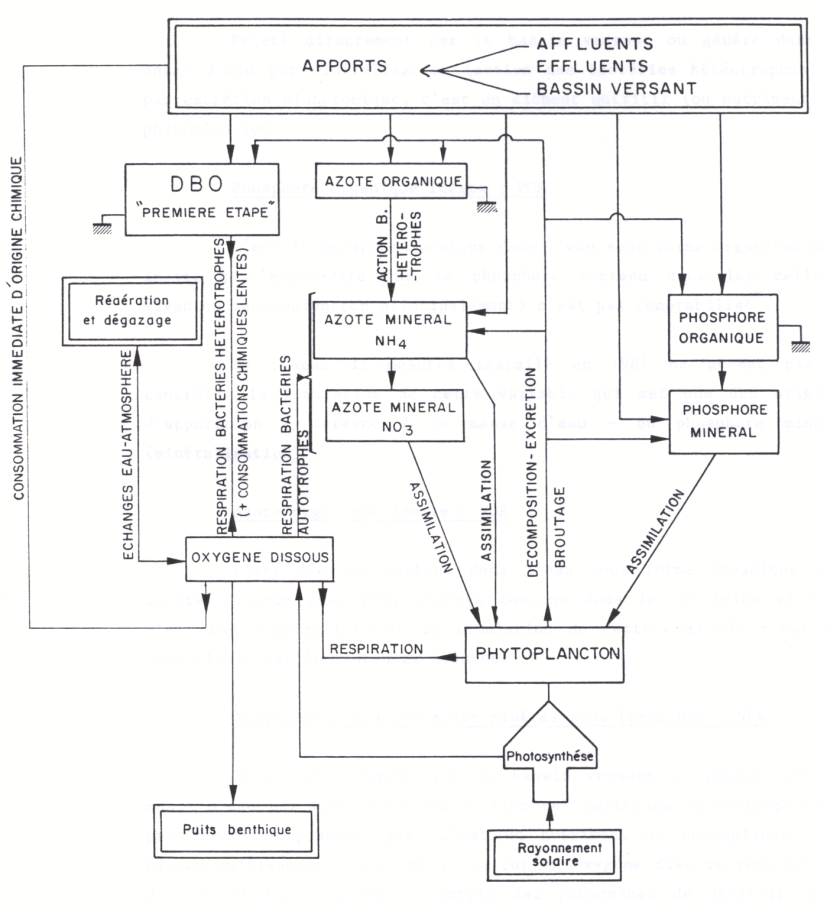
\includegraphics[scale=1.]{graphics/image38.png}
%  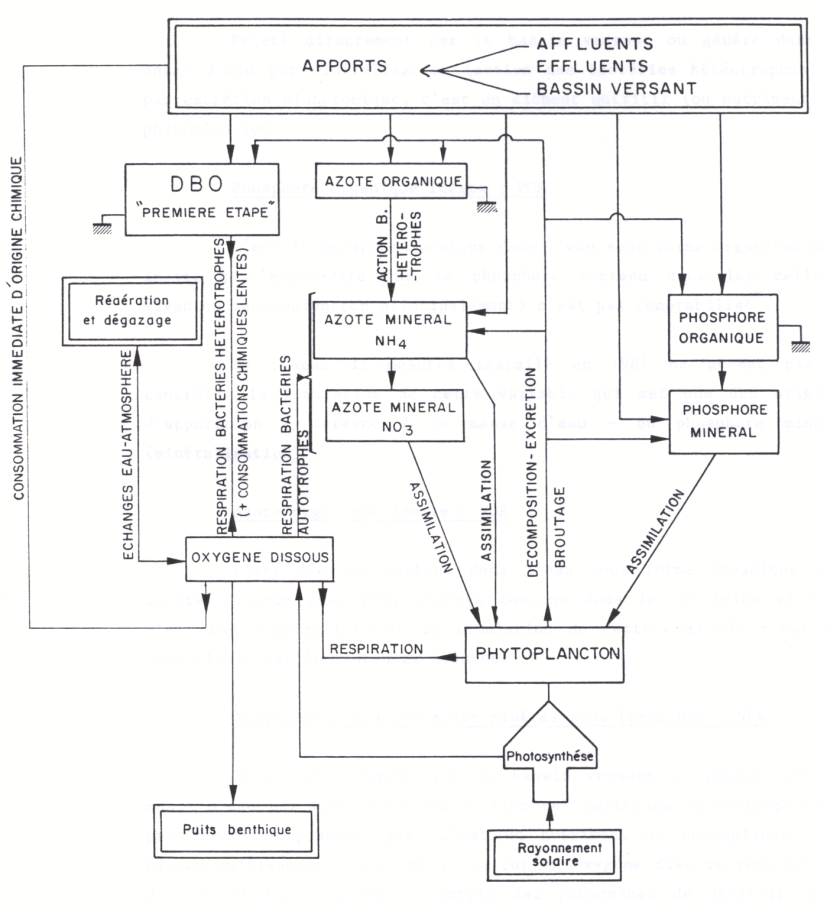
\includegraphics[width=3.76in,height=4.01in]{graphics/image38.png}
%  \caption{Schematic representation of the ecosystem modeled by the EUTRO module \cite{gosse_doubs_1989}.
%    Figure taken from \cite{elkadi_tracer_2012}.}
%  \label{ecosyst_scheme}
%\end{figure}

\section{Phytoplankton}

\subsection{Algal growth}

The algal growth rate $CP$ (d$^{-1}$) is given by
the exactly same equation as in BIOMASS module.
The parameters $C_{max}$
(\telkey{MAXIMUM ALGAL GROWTH RATE AT 20C}, default = 2),
$RAY$, $g_1$ and $\alpha_1$
(this last value can be chosen with the 1$^{\textrm{st}}$ value of the keyword
\telkey{ALGAL TOXICITY COEFFICIENTS}, default = 1 i.e. absence of toxicity)
are defined in the same way as in the BIOMASS module.

The parameters
\telkey{METHOD OF COMPUTATION OF RAY EXTINCTION COEFFICIENT} (default = 1~m$^{-1}$),
\telkey{VEGETAL TURBIDITY COEFFICIENT WITHOUT PHYTO} (default = 0~m$^{-1}$),
\telkey{PARAMETER OF CALIBRATION OF SMITH FORMULA} (default = 120~W/m$^2$),
\telkey{SUNSHINE FLUX DENSITY ON WATER SURFACE} (default = 0~W/m$^2$)
are still to be set as in BIOMASS.\\

The parameter representing the effects of phosphoric
and nitric nutrients on the algal growth $LNUT$ takes into account
the ammonia load assimilable by the phytoplankton NH$_4$ and is therefore defined by:

\begin{equation}
  LNUT = \min \left( \frac{[PO_4]}{KP+[PO_4]}, \frac{[NO_3]+[NH_4]}{KN+[NO_3]+[NH_4]} \right),
\end{equation}

with $KP$ half-saturation constant in phosphate
set with the keyword \telkey{CONSTANT OF HALF-SATURATION WITH PHOSPHATE}
(default = 0.005 mgP/l) as in BIOMASS,
and $KN$ half-saturation constant in nitrates
set with the keyword \telkey{CONSTANT OF HALF-SATURATION WITH NITROGEN}
(default = 0.03 mgN/l) as in BIOMASS.\\

\subsection{Algal disappearance}

The algal disappearance rate $DP$ (d$^{-1}$) is given
by the the same equation as in BIOMASS module.
\telkey{RESPIRATION RATE OF ALGAL BIOMASS}
(default = 0.05~d$^{-1}$) and the keyword
\telkey{COEFFICIENTS OF ALGAL MORTALITY AT 20C} (default = (0.1;0.003))
and \telkey{ALGAL TOXICITY COEFFICIENTS} (default = (1;0))
are still to be set as in BIOMASS.\\

The effect of temperature on algal disappearance
is represented by the function $g_2 = (1,050)^{T-20}$.

\section{Nitric and phosphoric nutrients}

The following physical and biochemical parameters are used to describe processes
influencing the evolution of nitric and phosphoric nutrients:

\begin{itemize}
\item \telkey{PROPORTION OF PHOSPHORUS WITHIN PHYTO CELLS}
  for the average proportion of phosphorus in the cells of living phytoplankton $fp$ (0.0025~mgP/$\mu$gChlA),
\item \telkey{PERCENTAGE OF PHOSPHORUS ASSIMILABLE IN DEAD PHYTO}
  for the proportion of directly assimilable phosphorus in dead phytoplankton $dtp$ (default = 0.5),
\item \telkey{RATE OF TRANSFORMATION OF POR TO PO4}
  for the transformation rate of POR into PO$_4$ through bacterial mineralization at 20$^{\circ}$C
  $k_{320}$ (default = 0.03~d$^{-1}$),
\item \telkey{RATE OF TRANSFORMATION OF NOR TO NO3}
  for the transformation rate of NOR into NO$_3$ through heterotrophic
  and autotrophic bacterial mineralization at 20$^{\circ}$C $k_{620}$ (default = 0~d$^{-1}$),
\item \telkey{PROPORTION OF NITROGEN WITHIN PHYTO CELLS}
  for the average proportion of directly assimilable nitrogen in living phytoplankton $fn$ (0.0035~mgN/$\mu$gChlA),
\item \telkey{PERCENTAGE OF NITROGEN ASSIMILABLE IN DEAD PHYTO}
  for the proportion of directly assimilable nitrogen in dead phytoplankton $dtn$ (default = 0.5),
\item \telkey{CONSUMED OXYGEN BY NITRIFICATION}
  for the quantity of oxygen consumed by nitrification $n$ (default = 5.2~mgO$_2$/mgNH$_4$),
\item \telkey{CONSTANT FOR THE NITRIFICATION KINETIC K520}
  for the kinetics of nitrification at 20$^{\circ}$C $k_{520}$ (default = 0.35~d$^{-1}$),
\item $F_{POR}$: deposition flux of non-algal organic phosphorus (g/m$^2$/s).
  $F_{POR} = W_{POR} [POR]$,
  $W_{POR}$ is the sedimentation velocity of non-algal organic phosphorus
  given by the keyword \telkey{SEDIMENTATION VELOCITY OF ORGANIC PHOSPHORUS}
  (default = 0~m/s),
\item $F_{NOR}$: deposition flux of non-algal organic nitrogen (g/m$^2$/s).
  $F_{NOR} = W_{NOR} [NOR]$, $W_{NOR}$ is the sedimentation velocity of non-algal organic nitrogen
  given by the keyword \telkey{SEDIMENTATION VELOCITY OF NON ALGAL NITROGEN}
  (default = 0~m/s).

\item $Rn$: proportion of nitrogen assimilated in the form of NH$_4$ = $\frac{[NH_4]}{[NH_4]+[NO_3]}$.
\end{itemize}

\section{Organic load}

The following physical and biochemical parameters are used to describe processes
influencing the evolution of the organic load ($L$):

\begin{itemize}
\item \telkey{CONSTANT OF DEGRADATION OF ORGANIC LOAD K120}
  for kinetic degradation constant for the organic load at 20$^{\circ}$C $k_{120}$
  (default = 0.35~d$^{-1}$),
\item $g_3 = (1.047)^{T-20}$: effect of temperature on the degradation of organic load,
\item $F_{LOR}$: deposition flux of the organic load (g/m$^2$/s) = $W_{LOR}$.[L],
  with $W_{LOR}$ the sedimentation velocity of the organic load
  given by the keyword \telkey{SEDIMENTATION VELOCITY OF ORGANIC LOAD}
  (default = 0~m/s).
\end{itemize}

\section{Dissolved oxygen}

The following physical and biochemical parameters are used to describe processes
influencing the dissolved oxygen balance (O$_2$):

\begin{itemize}
\item \telkey{OXYGEN PRODUCED BY PHOTOSYNTHESIS}
  for oxygen quantity produced by photosynthesis $f$
  (default = 0.15~mgO$_2$/$\mu$gChlA),
\item  \telkey{BENTHIC DEMAND} (default = 0.1~gO$_2$/m$^2$/d)
  for benthic oxygen demand $BEN$ (cf. O$_2$ model),
\item $k_2$: water-atmosphere gaseous exchange coefficient,
  also called reaeration coefficient, at 20$^{\circ}$C (d$^{-1}$).
  It can be provided by the user with the keyword
  \telkey{K2 REAERATION COEFFICIENT} (default = 0.9~d$^{-1}$)
  or calculated using formulae in the literature
  with the keyword \telkey{FORMULA FOR COMPUTING K2} (cf. O$_2$ module),
\item $g_4 = (1.025)^{T-20}$: effect of temperature on natural reaeration,
\item $C_s$: concentration of oxygen saturation in water (mgO$_2$/l).
  It can be determined from the water temperature
  with the formula chosen with the keyword
  \telkey{FORMULA FOR COMPUTING CS} (default = 0 i.e. constant value given by
  \telkey{O2 SATURATION DENSITY OF WATER (CS)}, default = 11~mg/l),
  cf. O$_2$ module.
%\item $r$: relationship defining the influence of weirs on oxygen concentration (cf. O$_2$ module)
\end{itemize}


% ??? \telkey{PHOTOSYNTHESIS P} (default = 1~mgO${}_{2}$/d/l)
